\section{Introduction}

%\begin{enumerate}
%\item{1} Bimanual manipulation-suturing is important and challenging
%\item{2} Our task is stent graft manufacturing
%%\item{3} Unsolved problems:Path planning,Adaptive to new context
%%\item{4} Our solutions:Vision + learn from demonstration,
%%Path planning - learning from demonstration, needle tracking, tool tracking,
%%Adaptive to new context - object centric approach + vision guided.
%\end{enumerate}
%~\cite{bidan2013grasp}
Sewing is a delicate and pain-stacking task. Recent development in robotics has largely increased the efficiency of the sewing industry. Most of these robotic solutions are specialised in one or a few certain types of machine stitches, such as the lock stitches. Some conventional hand stitches are hard to automate and still requires human labour. Our motivation of the study is to free human from the tiring sewing jobs and teach the robot to make hand stitches. Particularly, we focus on the task of personalized stent graft manufacturing.

A stent graft is a tubular structure composed of fabric supported by a metal mesh called stent. It is widely used for a variety of pathologies during endovascular interventions, such as reinforcing the vessel wall in presence of aneurysms.
Clinically, each stent graft needs to be customised to the patient anatomy, with fenestrations (openings) on the graft body to maintain the patency of side branches to vital organs. They often come at a significant cost in addition to a long manufacturing process. This is mainly due to the intensive manual tasks involved in the process. As a consequence, patients are more likely to be subjected of complications, e.g. aneurysm eruption, during the waiting period and precluding treatment to patients presenting acutely. Improved manufacturing of personalised stent grafts is therefore a critical unmet clinical demand and we are pursuing a robot assisted manufacturing approach. This study focuses on the key process of the stent graft manufacturing: sewing the stent to a fabric tube. For this purpose, a robotic system is proposed here in order to replicate the hand stitches required during the stent graft manufacturing process.



\begin{figure}
\centering
{
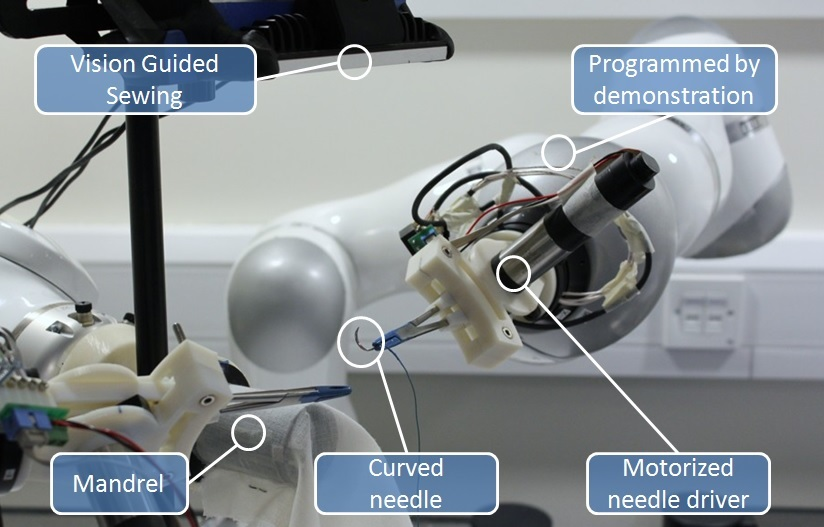
\includegraphics[width=8cm]{./fig/setup_label.jpg}
\caption{Robot sewing system for personalized stent graft manufacturing}
\label{fig:setup}}
\end{figure}

%Generally, stent grafts comprise two components: a quasi blood-tight textile tube called graft and a reinforcing metallic ring called stent. Clinically, each stent graft needs to be customised to the patient anatomy, with fenestrations (openings) on the graft body to maintain the patency of important branches to vital organs. Generally, hand sewing techniques are used to attach the reinforcing rings to the fabric and finishing the edge of a fenestration.
%The technique is very similar with the suturing used in medical filed, in which a circular needle and a needle holder are used. A personalized stent graft with complex shape requires employing with many hundreds or thousands of sutures. The time associates with attaching sutures for manufacturing a custom-made stent graft is long and the burden of assuring the quality of every stitch is also expensive. Currently, manufacturing one personalized stent graft tasks as long as take 6-12 weeks, for patient with complex dilemma, waiting for its delivery creates unparalleled health risk. The development of an automated or partially automated stent graft sewing technique would therefore be very helpful to change the status.

Automated sewing has been extensively researched in textile industry. Intelligent robotic systems with multi-sensor feedback are built to work in conjunction with a traditional sewing machine. Important topics in this filed includes bimanual robotic sewing~\cite{kudo2000multi}, fabric tension control, and seam tracking~\cite{schrimpf2012experiments, schrimpf2012real}. To cope with environmental changes during the sewing process, various control strategies are implemented, such as a fuzzy logic controller~\cite{koustoumpardis2006intelligent}, a hybrid position/force control~\cite{kudo2000multi}, a leader/follower control strategy~\cite{schrimpf2014velocity}. In addition, extensive research has been carried out in the design of sewing heads capable of access the sewn object from a single side, which allows the sewing to be performed on a 3D surface. For example, KSL Keilmann (Lorsch, Germany) has develop various 3D stitching systems incorporating single sided sewing heads onto KUKA manipulators for sewing fabric-reinforced structure of aircraft parts. These machines are designed for sewing large and heavy objects. Delicate sewing for small objects with non uniform shapes are still mainly hand made.

As the emerging of robotic assisted systems in the field of minimally invasive surgery, research on automated suturing tasks is also widely investigated, which provides the advantage of the machine speed and accuracy of the suturing process. A suturing task can be divided into two sub-tasks: tissue piercing and knot tying. For each task, research is carried by planning the procedure according to well established manual suture techniques~\cite{jackson2013needle,kapoor2008constrained, nageotte2005circular} or learning the skills from expert demonstrations ~\cite{padoy2011human, mayer2008system, van2010superhuman}. Vision guidance/visual servoing plays a key role in the achievement of a fully automated suturing task. In the aspect of positioning the needle to the target point, both the needle posture and the target suturing plane posture need to be measured. Iyer et al.~\cite{iyer2013single} proposed a single arm single camera system auto-suturing system in which the area being sutured on is marked by round markers. In their method, the monocular pose measurement algorithm ~\cite{lo2002trip} was used for estimating the needle posture. Another work presented by Staub et al.~\cite{staub2010automation} introduced 3D stereo system and visual servoing technique to improve the accuracy in aligning the needle with target stitching point. Recently, an auto-suturing system with 2D camera guidance and motorized Endo 360º suturing device is presented~\cite{leonard2014smart}. In this work, a method is presented to track incision contour and automatically distributes equally-spaced stitches along the incision.


\begin{figure}
\centering
{
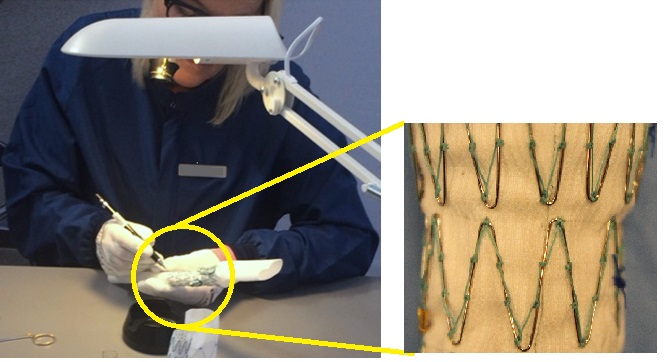
\includegraphics[width=8cm]{./fig/sewinglady.jpg}
\caption{A lady is hand sewing stent graft. The right image shows the stitches on a stent graft}
\label{fig:sewinglady}}
\end{figure}
%Comparing the techniques used in industrial sewing and surgical suturing, we found that the latter is more suitable for sewing a stent graft.
Inspired by these medical sewing approaches, we use robots to control a needle driver to manipulate a curved needle for sewing. Compare to conventional sewing machines, this approach is more versatile, allowing us to do stent sewing, fenestration finishing and knot tying with the same setup. A learning from human demonstration approach is used here so that the robot sewing movements can be programmed easily.

%Firstly, suturing with a circular needle and needle driver is versatile that can do both stent sewing, fenestration finishing and knot tying. In addition, the hand-made stitch type, like blanket stitch, is stronger than machine made double-thread stitch which easily comes out when one point breaks. Due to these reasons, we propose a framework in which the suturing skills of an expert could be transferred to a robot holding a needle driver and the robot is able to adapt even the needle posture is changed during needle grasping.

% Why single side sewing ? ---------------------------------
The use of curve needle also gives us the benefit of doing single sided sewing.
The shape of the fabric tube, i.e. the graft, is pre-designed for the patient anatomy and pre-manufactured. The tube can not be flattened into a single layer and hence conventional techniques of sewing a flat fabric is not applicable. Single sided sewing is an effective solution. Inspired by the conventional method of sewing stent grafts, we design a mandrel to support the fabric from the inside (Figure~\ref{fig:sewinglady}). Figure~\ref{fig:setup} shows our sewing system.
To ensure the stitch quality and the system robustness, we use a vision system to guide the sewing process. As far as we know, this is the first automotive sewing system that use curved needle to make hand stitches.

This paper presents the proposed system and is organized as follows. Section 2 describe our system, both the hardware design and the software components. Section 3 shows the experiments we conduct using this system and presnets the results, followed by the discussion in Section 4.

% Challenges and solutions ---------------------------


